\subsection{Pair Discovery}
\label{sec:local_join}
In this Section, we propose two solutions for the pair discovery problem. The first (Section~\ref{subsec:sweep_line_join}) is a baseline algorithm that uses a sweep line to scan the co-evolving time series throughout their duration, while validating and keeping all the pairs that satisfy the given constraints employing a value discretization scheme per timestamp (Section~\ref{subsec:indexing}). The second method (Section~\ref{subsec:checkpoint_join}) employs an optimization that reduces the number of pairs to consider by judiciously probing candidates at selected timestamp values (referred to as \textit{checkpoints}, Section~\ref{sec:checkpoint}). This significantly prunes the search space without missing any qualifying results.

%\checknote{A trivial solution to the pair discovery problem would involve the calculation of all the pairs at each timestamp and then cross-checking all possible pair combinations going from the axis origin and towards the rightmost timestamp. Given a set of time series $\mathcal{X}$ of length $k$, getting all the pairs at a specific timestamp has a complexity of $\mathcal{O}(|\mathcal{X}|!/2(|\mathcal{X}|-2)!)$, since we seek all possible combinations. Thus, cross-checking all possible pairs at each timestamp would result to an overall complexity of $\mathcal{O}([|\mathcal{X}|!/2(|\mathcal{X}|-2)!]^k)$, which is prohibitively expensive.}


\subsubsection{Value Discretization}
%\subsection{Indexing Value Axis}
\label{subsec:indexing}
To reduce the candidate pairs that need be checked at each timestamp $t$, we discretize the values of all time series at $t$ in {\em bins}, i.e., several consecutive value ranges, each one of size $\epsilon$. Time series with values within the same bin at timestamp $t$ form candidate pairs, but we also need to check adjacent bins for additional candidate pairs whose values differ by at most $\epsilon$. Time series having values at non-adjacent bins are certainly farther than $\epsilon$ at that specific timestamp $t$, so we can avoid these checks. 

To detect all candidate pairs and avoid cross-checking in every two adjacent bins we consider a \textit{value range} of size $\epsilon$, whose upper endpoint coincides with each value under consideration at time $t$. Then, all values of time series contained within this range, form candidate pairs (see Figure~\ref{fig:index}). Obviously, values contained in the same bin $j$ can form candidate pairs. Then, we can cross-check each value in bin $j$ with values in bin $j+1$ for additional candidates with value difference at most $\epsilon$, as indicated with the red (right) range.


\begin{figure}[tb]
    \centering
    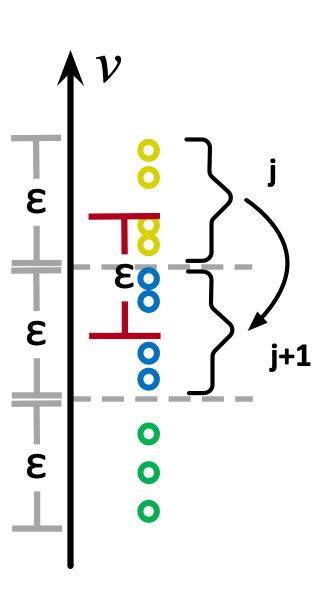
\includegraphics[width=0.12\textwidth]{figures/index.png}
    \caption{Discretization of time series values at timestamp $t$.}
    \label{fig:index}
\end{figure}

At each timestamp $t$, the process of finding all the pairs consists of: (1) \textit{Filtering} - Search among time series values in adjacent bins to detect candidate pairs using the aforementioned search method. (2) \textit{Verification} - For each candidate pair, check similarity of their respective values at successive timestamps as long as this pair still qualifies to the matching conditions (or the end of time series data is reached). This step resembles to a ``horizontal expansion'' along the time axis in an attempt to eagerly verify and report pairs.

\subsubsection{Pair Discovery Using Sweep Line}
\label{subsec:sweep_line_join}
A baseline method for pair discovery over a set of time series is to check all the candidate pairs formed at each timestamp, and verify whether the minimum duration constraint $\delta$ is satisfied. Algorithm \ref{alg:simple_scan_sim} describes this procedure. Pair discovery (Line 5) considers a time duration $T$ (as a set of consecutive timestamps) to check for results. Initially $T = \{0, \dots, k\}$, where $k$ is the total duration of all time series data. For each timestamp $t$, we obtain only the subset of time series whose values are contained in two adjacent bins (Line 7). Based on these values at $t$, we obtain all candidate pairs with respect to the threshold $\epsilon$ (Line 9). For each such pair, if it is not already part of the resulting pairs at that specific timestamp $t$, we \textit{verify} it by first expanding it horizontally (Lines 10-12) and checking whether this pair meets the duration constraint $\delta$ (Line 13) along subsequent timestamps. If so, we add it to the reported results (Line 14).

For the \textit{horizontal expansion}, we iterate over the subsequent timestamps (after the current one -- Line 17) and stop when $\epsilon$ is violated (Lines 18--19). Then, we mark the start of this pair with the current timestamp $t$, whereas its end is marked by the timestamp at which $\epsilon$ is crossed, and we return this pair (Lines 20-22).

\SetKwInOut{Parameter}{Parameters}

\setlength{\textfloatsep}{4pt}
\begin{algorithm}[tb]
	\DontPrintSemicolon
	\begin{footnotesize}
	\KwIn{Set $\mathcal{X}$ of co-evolving time series of length $k$}
	\nonl \textbf{Parameters}: Threshold $\epsilon$, min duration $\delta$ \\
	\KwOut{List $P$ with all locally similar pairs of time series}
	\vspace{4pt}
	
	
	$B \leftarrow CreateBins(\mathcal{X})$ \\
	$P \leftarrow DiscoverPairs(\emptyset, B, \{0, ..., k\}, \epsilon, \delta)$ \\
	\KwRet $P$
	
	\vspace{4pt}
	\SetKwProg{procFilter}{Procedure}{}{}
	\procFilter{$DiscoverPairs(P, B, T, \epsilon, \delta)$}{
    	\ForEach{$t \in T$}{
            \ForEach{$z=0 \to B.size$}{
                $\mathcal{X}' \leftarrow B^t_z \cup B^t_{z+1}$ \\
                \ForEach{$X \in \mathcal{X}'$}{
        	        $\mathcal{P}^t \leftarrow getAdjacentPairs(X^t, \epsilon)$ \\
        	        \ForEach{$p \in \mathcal{P}^t$} {
        	            \If{$p \notin P$}{
        	                $p \leftarrow VerifyPair(p, t, k, \epsilon)$ \\
        	                \If{$p.end-p.start \geq \delta$}{
        	                    $P \leftarrow P \cup p$ \\
        	                }
        	            }
        	        }
        	    }
    	    }
    	}
    	\KwRet $P$ \\
	}
	
	\vspace{4pt}
	\SetKwProg{procExpand}{Procedure}{}{}
	\procExpand{$VerifyPair(p, t, k, \epsilon)$}{
	    \ForEach{$t'=t+1 \to k$}{
	        \If{$|p.X_i^{t'}-p.X_j^{t'}| > \epsilon$}{
	            $break$ \\
	        }
	    }
	    $p.start \leftarrow t$ \\ 
	    $p.end \leftarrow t'$ \\ 
		\KwRet $p$ \\
	}
	\end{footnotesize}
	\caption{Sweep line scan pair discovery}
	\label{alg:simple_scan_sim}
\end{algorithm}


However, searching over all timestamps in such an exhaustive manner can be expensive, particularly for long time series. Next, we present an optimization that identifies candidate pairs at selected timestamps only, so that only those pairs require verification.

\subsubsection{Optimized Filtering at Checkpoints}
%\subsection{Optimization with Checkpoint Filtering}
\label{sec:checkpoint}

To prune the search space, we consider \textit{checkpoints} along the time axis, so that searching for candidate pairs will be performed at these specific timestamps only. If the temporal span between two successive checkpoints does not exceed the minimal duration threshold $\delta$, we can ensure no false negatives, since any qualifying pair starting at an intermediate timestamp between two checkpoints will surely be detected at least on the second one. Figure \ref{fig:checkpoints} shows an example for a set of time series (checkpoints placed every $\delta=5$ timestamps).

\begin{figure}[tb]
    \centering
    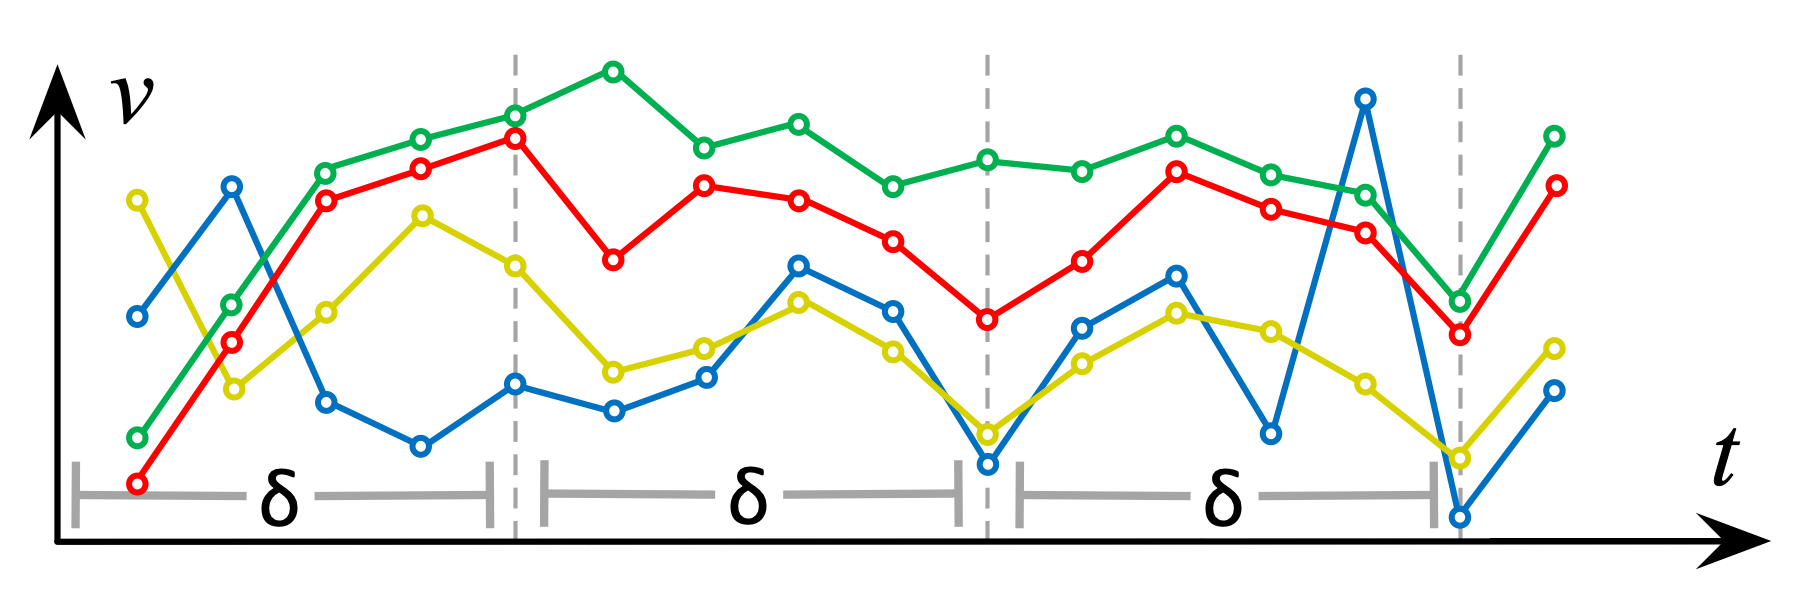
\includegraphics{figures/checkpoints.png}
    \caption{Checkpoints placed every $\delta$ timestamps.}
    \label{fig:checkpoints}
\end{figure}

Assume a set of checkpoints placed at time interval $\delta$ from each other, as depicted in Figure \ref{fig:proof1}. Let a checkpoint at timestamp $t'$ and a qualifying pair of duration $\delta$ starting at timestamp $t'-\delta+1$. This pair cannot have smaller duration, otherwise it would not meet constraint $\delta$. Consequently, the pair will be detectable on the checkpoint at $t'$, as shown in the figure. Similarly, if a qualifying pair ends at timestamp $t'+\delta-1$ (Figure \ref{fig:proof2}), it will be detected at the checkpoint at $t'$. Hence, all pairs around a checkpoint at $t'$ can be detected as candidates when we check their values at $t'$. Thus, we can easily conclude to the following observation.

\begin{mylemma}[Checkpoint Covering Interval]
Let the interval between successive checkpoints not exceed $\delta$. Considering a checkpoint placed at timestamp $t'$, all qualifying pairs starting at $s, t'-\delta+1 \leq s < t'$ and ending at $f, t' < f \leq t'+\delta-1$ will satisfy all matching constraints at timestamp $t'$.
\end{mylemma}


\begin{figure}[!t]
 \centering
 \subfloat[Pair with a starting point before $t'$.]{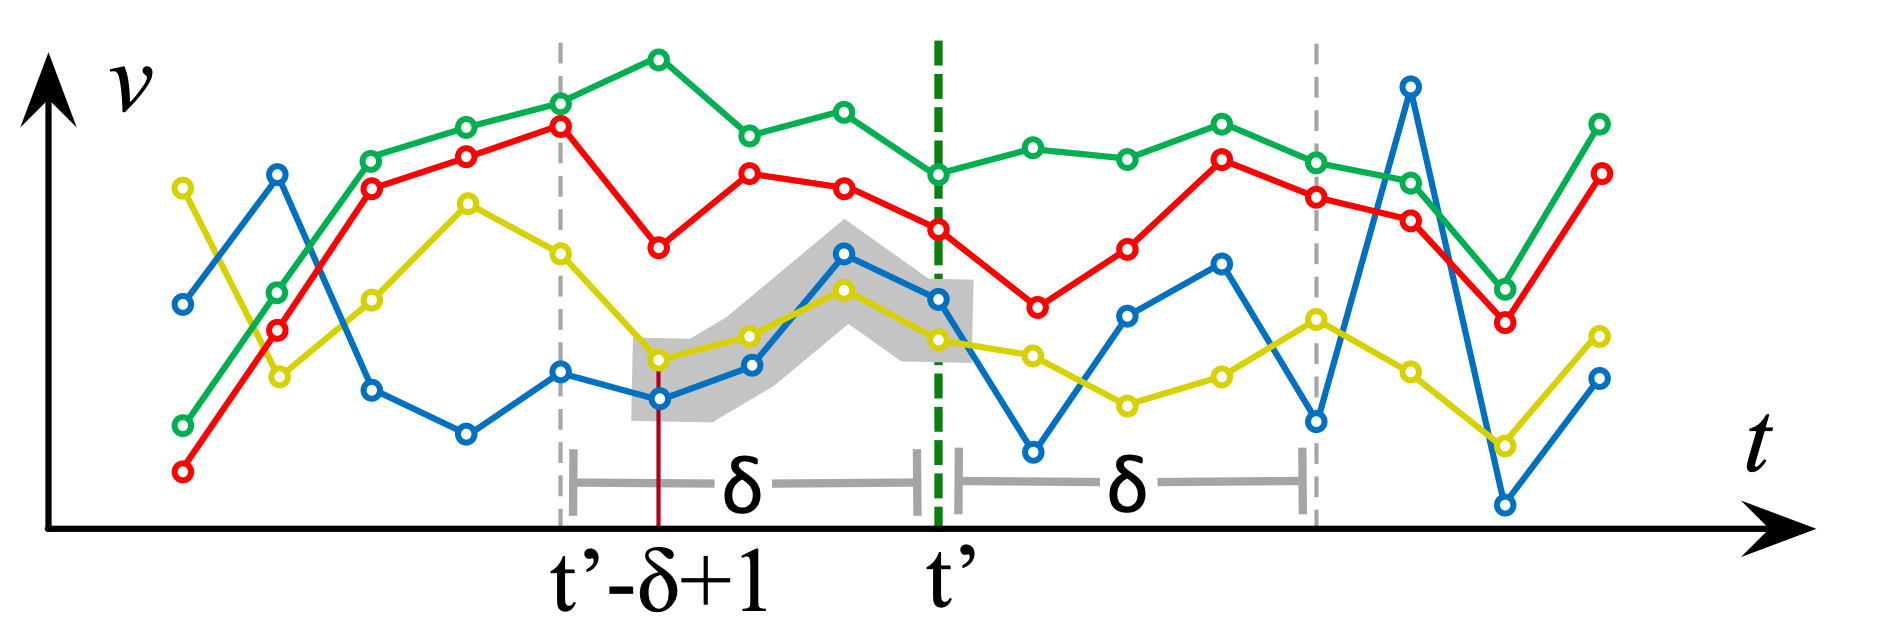
\includegraphics[width=0.43\textwidth]{figures/proofLeft.png}\label{fig:proof1}}
 \subfloat[Pair with an ending point after $t'$.]{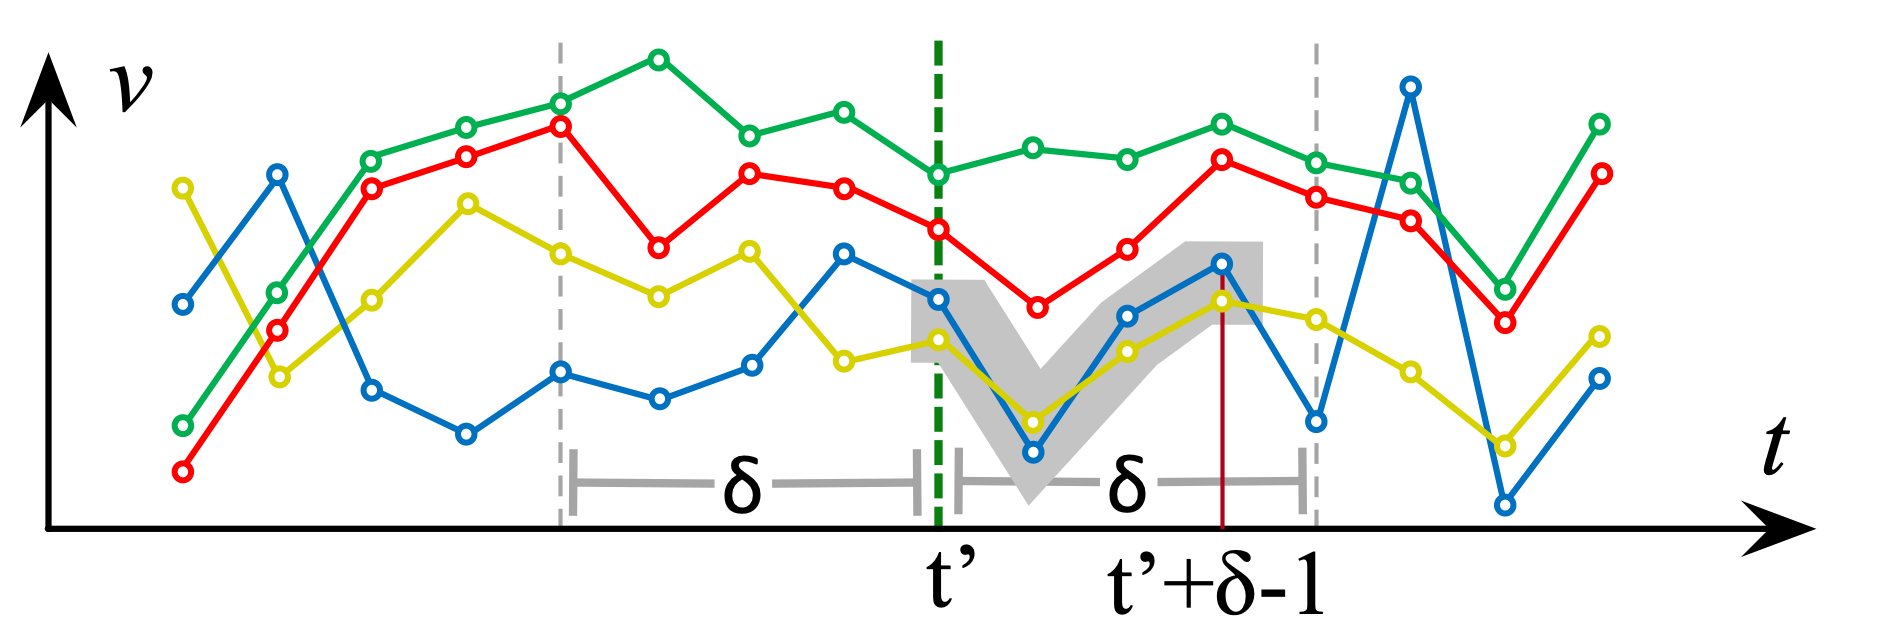
\includegraphics[width=0.43\textwidth]{figures/proofRight.png}\label{fig:proof2}}
 \caption{A qualifying pair will be detected on a checkpoint.}
 \label{fig:proof}
\end{figure}


This lemma entails that it suffices to check for candidate pairs only at checkpoints, i.e., every $\delta$ timestamps. We denote the set of checkpoints as $C$. Since we skip timestamps and in order to avoid false misses, we now have to verify pairs with a horizontal expansion (as in \ref{subsec:sweep_line_join}), but towards both directions, i.e., before and after a given checkpoint. Overall, at each checkpoint the optimized process performs: (1) \textit{Filtering} - Search for candidate pairs among the values of time series in adjacent bins. (2) \textit{Verification} - For each pair, perform a \textit{two-way} horizontal expansion across the time axis.

% \begin{itemize}
%     \item \textbf{Filtering}: Search among the values of time series in adjacent bins to detect candidate pairs.
%     \item \textbf{Verification}: For each candidate pair, perform a \textit{two-way} horizontal expansion across the time axis.
% \end{itemize}

\paragraph{Improving placement of checkpoints} Depending on the dataset, the default checkpoint placement might yield an \textit{increased} number of candidate pairs, resulting in too many verifications. Intuitively, if the time series values at a specific timestamp $t'$ are placed in a more \textit{``scattered''} manner over the bins, less candidates would be generated. This is because the values of time series at $t'$ would differ from each other by more than $\epsilon$ and thus can be pruned as described in Section \ref{subsec:indexing}. Figure \ref{fig:opt1} depicts such a case of sub-optimal placement of checkpoints, where the second checkpoint is placed at a rather \textit{dense} area and as a result, six candidate pairs are considered. We can avoid this by shifting all checkpoints together either to the left or to the right, yet maintaining their temporal span every $\delta$. As shown in Figure \ref{fig:opt2}, all three checkpoints are collectively shifted to the left, avoiding the dense area and reducing the total number of candidate pairs. An extra checkpoint can be inserted before the first or after the last one, guaranteeing that there is no interval longer than $\delta$ without checkpoints.

%to the left (or to the right) in the case that we move the checkpoints so that the distance among the first timestamp and the first checkpoint (or the last timestamp and the last checkpoint) becomes more than $\delta$.

\begin{figure}[tb]
    \centering
    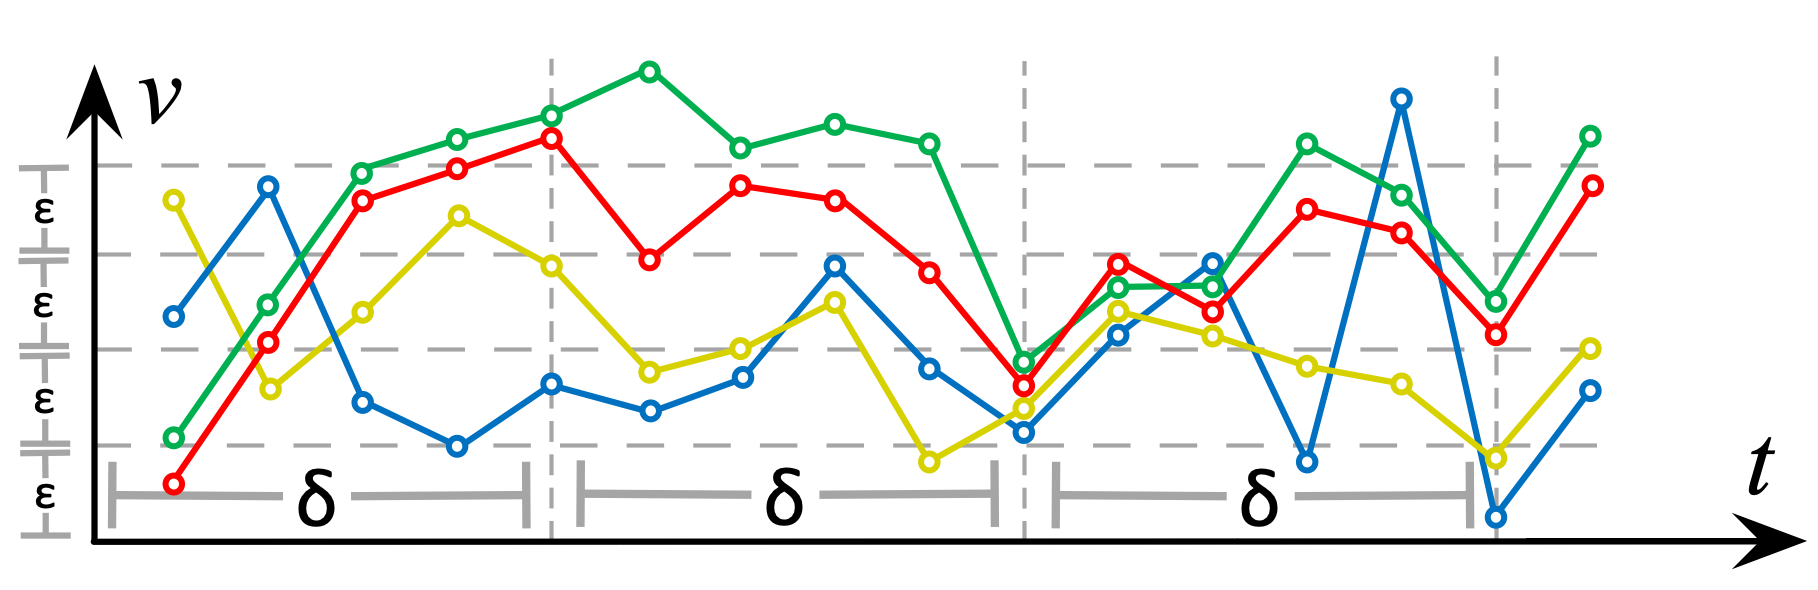
\includegraphics{figures/sub_opt.png}
    \caption{Sub-optimal checkpoint placement.}
    \label{fig:opt1}
\end{figure}

\begin{figure}[tb]
    \centering
    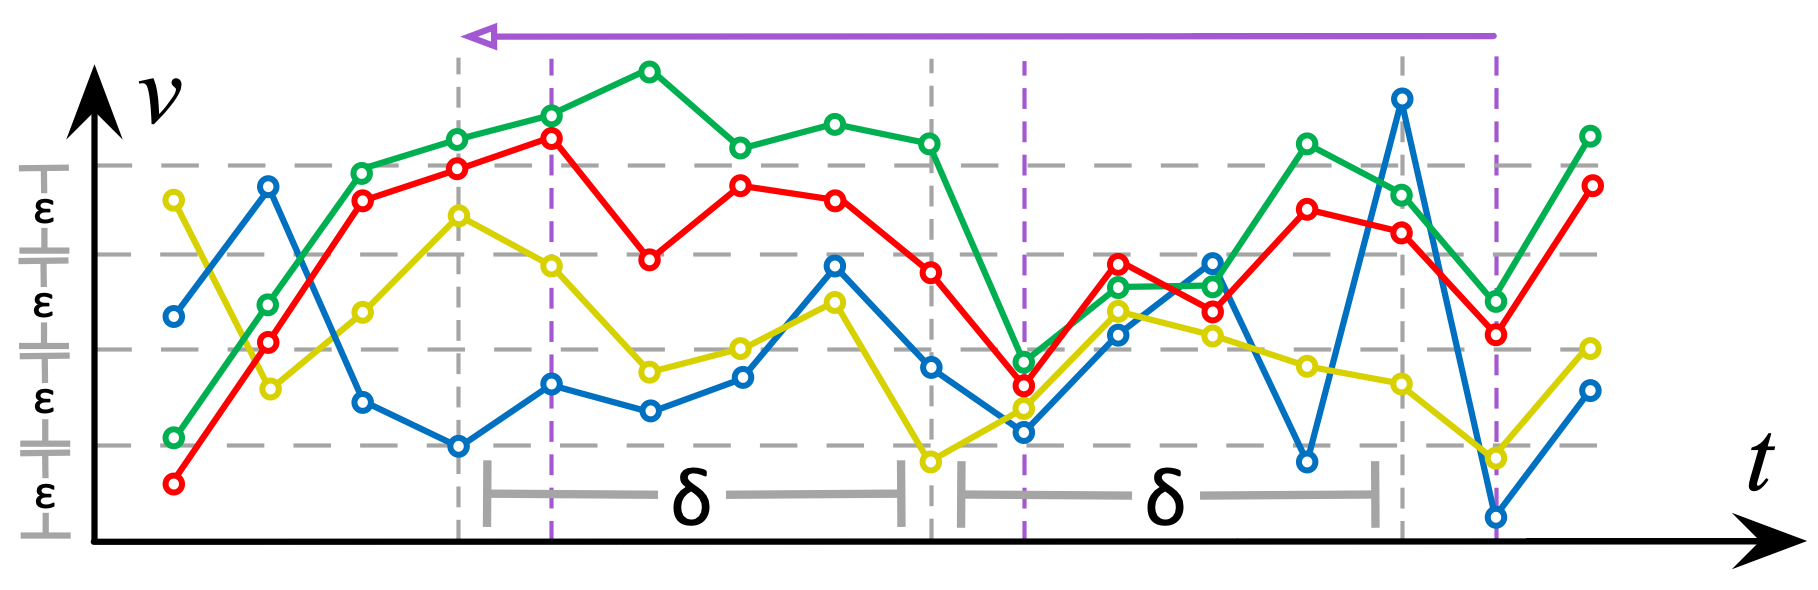
\includegraphics{figures/opt.png}
    \caption{Improved checkpoint placement.}
    \label{fig:opt2}
\end{figure}

Clearly, the placement of the set $C$ of checkpoints influences the amount of candidate pairs. We wish to find the best such placement, which provides the least number of candidate pairs. The amount of candidates depends on the cardinality of the bins (i.e., the number of values in each one, as shown in Fig.~\ref{fig:index}) at any particular checkpoint $c \in C$. Given that $n$ is the total number of time series in the dataset (and hence the number of values at each checkpoint), we can identify the most populated bin at checkpoint $c$ by calculating the maximal density $\frac{\max\{B_{c}\}}{n}$, where $B_{c}$ represents the set of bin cardinalities at checkpoint $c$. Therefore, for a given configuration $C$ of checkpoints, we can estimate an overall cost $r$ by taking the sum of such maximal densities over all checkpoints, i.e.,  $r=\sum_{c \in C}{\frac{\max\{B_{c}\}}{n}}$. The less this total cost, the smaller the cardinality per bin at each checkpoint and, thus, the less the candidates that will be generated. Consequently, we seek to find the minimum $r$. To do so, we shift all checkpoints together to the right, one timestamp at a time, we estimate ratio $r$ again and repeat $\delta$ times. This procedure is illustrated in Figure \ref{fig:heuristic1}, where the checkpoints symbolized with similar lines belong to the same set as we move them to the right in order to identify the best placement (indicated with the thickest vertical dashed lines).

\begin{comment}
To find the best checkpoint placement, we consider a cost, calculated by adding together the per checkpoint \textit{most populated bin size} over \textit{dataset size} ratio, i.e., $r=\sum{[(\max{B_{\omega_i}})/n}]$, where $B_{\omega_i}$ is the set of bins at checkpoint $\omega_i$ and $n$ the size of the dataset. 
\end{comment}

\begin{figure}[tb]
    \centering
    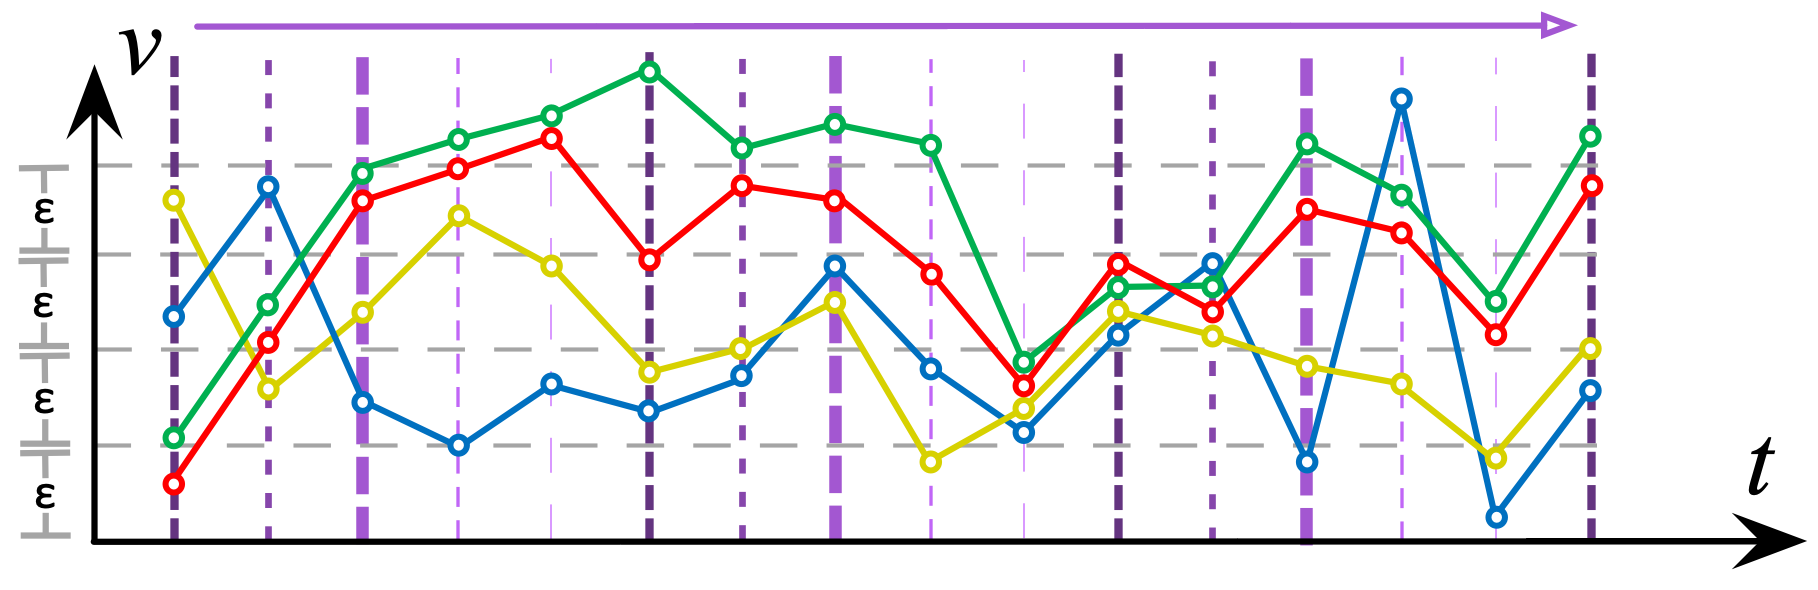
\includegraphics{figures/heuristic.png}
    \caption{Best checkpoint placement (thick vertical lines).}
    \label{fig:heuristic1}
\end{figure}


\setlength{\textfloatsep}{4pt}
\begin{algorithm}[tb]
	\DontPrintSemicolon
	\begin{footnotesize}
	\KwIn{Set $\mathcal{X}$ of co-evolving time series of length $k$}
	\nonl \textbf{Parameters}: Threshold $\epsilon$, min duration $\delta$ \\
	\KwOut{A list $P$ containing all the locally similar time series}
	\vspace{4pt}
	
	$B \leftarrow CreateBins(\mathcal{X})$ \\
	$C \leftarrow GetCheckpoints(k, \delta)$ \\
	$P \leftarrow DiscoverPairs(\emptyset, B, C, \epsilon, \delta)$ \\
	\KwRet $P$ \\
	
	\vspace{4pt}
	\SetKwProg{procVerify}{Procedure}{}{}
	\procVerify{$VerifyPair2Way(p, t, k, \epsilon)$}{
	    \ForEach{$t'=t-1 \to 0$}{
	        \If{$|p.X_i^{t'}-p.X_j^{t'}| > \epsilon$}{
	            $break$ \\
	        }
	    }
	    $p.start \leftarrow t'$ \\
	    $t_c \leftarrow p.start + \delta - 1$ \\
	    \ForEach{$t'=t_c \to t$}{
	        \If{$|p.X_i^{t'}-p.X_j^{t'}| > \epsilon$}{
	            $p.f \leftarrow t$\\
	            \KwRet $p$ \\
	        }
	    }
	    \ForEach{$t'=t_c+1 \to k$}{
	        \If{$|p.X_i^{t'}-p.X_j^{t'}| > \epsilon$}{
	            $break$ \\
	        }
	    }
	    $p.end \leftarrow t'$ \\
		\KwRet $p$ \\
	}
	\end{footnotesize}
	\caption{Checkpoint scan pair discovery}
	\label{alg:checkpoint_scan_sim}
\end{algorithm}


\subsubsection{Pair Discovery Using Checkpoints}
\label{subsec:checkpoint_join}
After identifying the best checkpoint placement, we can discover pairs of locally similar time series by applying the exhaustive algorithm presented in Section~\ref{subsec:sweep_line_join}, but iterating over the defined checkpoints instead of all timestamps. To speed up the verification step, we introduce an optimization that reduces the number of checks. For each candidate pair $p$ that started at (a possibly previous) timestamp $p.start$, we first expand its verification to the left. In case the current duration of pair $p$ is still less than $\delta$, we jump at timestamp $p.start + \delta$ in order to eagerly prune candidates that will not last at least $\delta$. There, we check directly whether the values of these two time series qualify, and we continue this check backwards in time. If at an intermediate timestamp the $\epsilon$ constraint is not met, we can stop the verification process and discard the candidate pair.

The procedure for pair discovery is listed in Algorithm \ref{alg:checkpoint_scan_sim}. Initially, we calculate the best possible checkpoint set (Line 2). Then, we run the procedure described in Section \ref{subsec:sweep_line_join} but instead of probing over all timestamps we iterate over the resulting checkpoint set (Line 3).

Regarding verification, we first move towards the leftmost endpoint (Line 6) and detect the starting timestamp of the pair (Line 9). Then, we iterate from the timestamp $t_c = p.start + \delta$ towards the initial timestamp $t$ (Line 11). If the pair does not qualify at a timestamp during this interval (Line 12), we set $t$ as its final timestamp and return the pair (Line 14). Otherwise, we continue from timestamp $t_c$ and towards the rightmost timestamp until the pair ceases to qualify (Lines 15-19).

\textbf{Cost analysis.} Let $N_{tc}$ be the number of examined timestamps (i.e., checkpoints) considered by the algorithm. For each such timestamp, the algorithm needs to perform two operations, namely first to generate the set of candidate pairs and second to verify each pair. Let $C_{cg}$, $C_{cv}$ and $N_c$ denote, respectively, the candidate generation cost, the verification cost per candidate and the number of generated candidates. Then, the total cost is $C = N_{tc} \times (C_{cg} + N_c \times C_{cv})$. The candidate generation cost $C_{cg}$ is proportional to the number of candidates $N_c$, which in turn is $\mathcal{O}(|\mathcal{X}|^2)$. However, in practice, the algorithm only needs to generate candidate pairs from the time series corresponding to the same bin. Let $\beta$ denote the number of bins ($\beta \leq (y_{max} - y_{min}) / \epsilon$) and $N_{\beta}$ the maximum number of time series associated with any bin. Then, the expected cost in practice would be $\beta \times N_{\beta}^2$. As $\epsilon$ increases, $\beta$ decreases but $N_{\beta}$ increases (in the worst case, $N_{\beta} = |\mathcal{X}|$, i.e., there is a single bin that contains all time series). Moreover, any candidate that has been already generated and verified in a previous timestamp need not be verified again, so the number of candidate pairs to be verified in the worst case is $\mathcal{O}(|\mathcal{X}|^2)$. Regarding the verification cost $C_{cv}$, consider a pair of time series $(X_i, X_j)$ that is generated at timestamp $\tau$. The algorithm needs to check for each subsequent timestamp $t \in (\tau, k)$ whether $|X_i^{t} - X_j^{t}| \leq \epsilon$, as long as this condition holds; hence, the cost is $\mathcal{O}(k)$. Of course, in practice, this will also require much fewer comparisons in most cases. Notice that the difference between Algorithm \ref{alg:checkpoint_scan_sim} and Algorithm \ref{alg:simple_scan_sim} is that the former generates and verifies candidates only at checkpoints, i.e., $N_{tc} = k / \delta$, while the latter at every timestamp, i.e., $N_{tc} = k$.

\subsection{Bundle Discovery}
\label{sec:bundle_disc}
We now consider the bundle discovery problem. We propose two algorithms: an exhaustive one using a sweep line (Section~\ref{subsec:sweepline_bundle}), and one using checkpoints (Section~\ref{sec:checkpoint_bundle}), following the same principles as in pair discovery.

%\checknote{Following a similar logic as in pair discovery, a trivial solution to the bundle discovery problem would involve obtaining all possible bundles at each timestamp and then cross-checking all possible combinations starting from the origin and going rightward. Again, given a set of time series $\mathcal{X}$ of length $k$, calculating all possible bundles of size at least $\mu$ at a specific timestamp, this time has a complexity of $\mathcal{O}(|\mathcal{X}|!/\mu(|\mathcal{X}|-\mu)!)$, since we now seek groups of size $\mu$. Consequently, the overall complexity would be $\mathcal{O}([|\mathcal{X}|!/\mu(|\mathcal{X}|-\mu)!]^k)$.}

%However, during the \textit{filtering} step along the value axis, all time series values within the $\epsilon$ range from a specific value form a candidate bundle (instead of many candidate pairs). Generation and best placement of checkpoints are the same as in pair discovery. The \textit{verification} step applies the same idea of horizontal expansion, but differs in the way it operates for bundles.

\subsubsection{Bundle Discovery Using Sweep Line}
\label{subsec:sweepline_bundle}
To exhaustively detect bundles of time series, we can follow a similar procedure employing a sweep line as in Section \ref{subsec:sweep_line_join}. However, this time we detect candidate bundles at each timestamp before verifying whether constraints concerning minimal duration $\delta$ and minimum membership $\mu$ are satisfied. Essentially, this can be thought of as an adaptation of the flock discovery approach in \cite{vieira2009line} to the 1-dimensional setting in the case of time series.
%To detect all candidate bundles and avoid cross-checking all values in every two consecutive bins, we adapt the logic from \cite{vieira2009line}, which is applied for detecting flocks of moving objects. In that case, it is proven that there is a limited and discrete number of locations to search for such flocks per timestamp. More specifically, the flock can be captured by a disc with diameter $\epsilon$ that covers all such locations. Since the center of such a disc can have infinite possible placements (all with diameter $\epsilon$) and still cover all object locations, they pick a disc having at least two of these locations on its circumference. 

%, by coinciding each point with one of the endpoints of the $\epsilon$ interval, as previously described. If the results do not contain any bundles that are the same, or cover (i.e., their members are a superset of the candidate at that timestamp) the candidate (Line 10), we check whether the number of contained time series satisfies the $\mu$ constraint (Line 11) and if so, we verify by expanding the bundle vertically rightwards (Line 12).

Algorithm \ref{alg:simple_scan_bundle} describes this exhaustive process. Similarly to pair discovery, at each timestamp $t$ (Line 5) we obtain only the values of time series contained in adjacent bins (Lines 6--7). Then, each such value is considered the origin of a search range $\epsilon$, which returns a candidate group at time $t$ (Line 9). Of course, such a candidate group may have been already included in the result bundles previously, during a horizontal expansion at a previous timestamp. In this case, its examination is skipped. Otherwise, if this group contains more than $\mu$ members, we proceed to verify it as a candidate bundle over subsequent timestamps via horizontal expansion (Lines 10-12). As will see next, this expansion may return one or more candidate bundles; each one is checked against the duration constraint $\delta$ before adding it to the result bundles (Lines 13-16).

Regarding the verification step of a candidate bundle $\mathcal{G}^t$, we apply its horizontal expansion over all subsequent timestamps (Line 19). For each member of such candidate bundle (Lines 21-28), we find the group $\mathcal{G}^{t'}$ of time series having values within range $\epsilon$ at time $t'$. Many such new groups may be created, as each member may yield one group. Such a group $\mathcal{G}^{t'}$ may become a new candidate bundle if it satisfies the $\mu$ constraint; if so, it is added to the resulting bundles with an updated duration (Lines 24--27). As we look at subsequent timestamps, it may happen that the same bundle may be added to the results multiple times, but with increasing duration. In the end, we eliminate duplicates and only keep the one with the longest duration (Line 28). Expansion stops once no new candidate bundles can be found in the next timestamp (Lines 29--30).


%At each timestamp $t'$, we loop over the current candidate bundles (Line 21).  

%\checknote{To support a leftward expansion for the checkpoint version, we check whether the rightmost timestamp is larger from the initial one (expansion to the right), or vice versa (expansion to the left) and update the starting and ending timestamps accordingly (Lines 27-30).} 

\setlength{\textfloatsep}{4pt}
\begin{algorithm}[ht!]
	\DontPrintSemicolon
	\begin{footnotesize}
    \KwIn{Set $\mathcal{X}$ of co-evolving time series of length $k$}
	\nonl \textbf{Parameters}: Threshold $\epsilon$, min duration $\delta$, min members $\mu$ \\
	\KwOut{A list $P$ containing all the discovered bundles}
	\vspace{4pt}
	
	$B \leftarrow CreateBins(\mathcal{X})$ \\
	$P \leftarrow DiscoverBundles(\emptyset, B, \{0, ..., k\}, \epsilon, \delta, \mu)$ \\
	\KwRet $P$
	
	\vspace{4pt}
	\SetKwProg{procFilter}{Procedure}{}{}
	\procFilter{$DiscoverBundles(P, B, T, \epsilon, \delta, \mu)$}{ 
	    \ForEach{$t \in T$}{
            \ForEach{$z \to B.size$}{
                $\mathcal{X}' \leftarrow B^t_z \cup B^t_{z+1}$ \\
        	    \ForEach{$X \in \mathcal{X}'$}{
        	        $\mathcal{G}^t \leftarrow getAdjacent(X^t, \epsilon)$ \\
        	        \If{$\mathcal{G}^t \notin P$} {
        	            \If{$\mathcal{G}^t.size \geq \mu$} {
        	                $\mathcal{B} \leftarrow VerifyBundle(\mathcal{G}^t, \{t, .., k\}, \epsilon, \mu)$ \\
        	                \ForEach{$\mathcal{G} \in \mathcal{B}$}{
        	                    \If{$\mathcal{G}.end-\mathcal{G}.start \geq \delta$}{
        	                        $P \leftarrow P \cup \mathcal{G}$
        	                    }
        	                }
        	            }
        	        }
        	    }
    	    }
	    }
	    \KwRet $P$ \\
	}
	
	\vspace{4pt}
	\SetKwProg{procVerify}{Procedure}{}{}
	\procVerify{$VerifyBundle(\mathcal{G}^t, \{t_1, ..., t_\phi\}, \epsilon, \mu, f)$}{
	    $P \leftarrow \mathcal{G}^t$ \\
	    \ForEach{$t'=t_2 \to t_\phi$}{
	        $expanded \leftarrow False$ \\
	        \ForEach{$\mathcal{G} \in P$}{
	            %$expanded \leftarrow False$ \\
                \ForEach{$X \in \mathcal{G}$}{
                    $\mathcal{G}^{t'} \leftarrow getAdjacent(X^{t'}, \epsilon)$ \\
                    \If{$(\mathcal{G}^{t'}.size \geq \mu$} {
                        Rearrange duration of $\mathcal{G}^{t'}$ accordingly\\
                        $P \leftarrow P \cup \mathcal{G}^{t'}$ \\
                        %\If{$t_\phi \geq t_1$}{
                        %    $\mathcal{G}^{t'}.start \leftarrow t_1, \mathcal{G}^{t'}.end \leftarrow %t'$ \\
                        %}
                        %\Else {
                        %    $\mathcal{G}^{t'}.start \leftarrow t', \mathcal{G}^{t'}.end \leftarrow %t_1$ \\
                        %}
                        $expanded \leftarrow True$ \\
                    }
                }
                $P \leftarrow keepLongestBundles(P)$
                %\If{$expanded=True$}{
                %    $P.remove(\mathcal{G})$
                %}
	        }
            \If{$expanded=False$}{
                $break$
            }
	    }
		\KwRet $P$ \\
	}
	\end{footnotesize}
	\caption{Sweep line scan bundle discovery}
	\label{alg:simple_scan_bundle}
\end{algorithm}



\begin{algorithm}[ht!]
	\DontPrintSemicolon
	\begin{footnotesize}
	\KwIn{Set $\mathcal{X}$ of co-evolving time series of length $k$}
    \nonl \textbf{Parameters}: Threshold $\epsilon$, min duration $\delta$, min members $\mu$ \\
	\KwOut{A list $P$ containing all the discovered bundles}
	\vspace{4pt}
	
	$B \leftarrow CreateBins(\mathcal{X})$ \\
	$C \leftarrow GetCheckpoints(k, \delta)$ \\
	$P \leftarrow DiscoverBundles(\emptyset, B, C, \epsilon, \delta, \mu)$ \\
	\KwRet $P$ \\
	
	\vspace{4pt}
	\SetKwProg{procVerify}{Procedure}{}{}
	\procVerify{$VerifyBundle2Way(\mathcal{G}^t, t, k, \epsilon, \mu)$}{
	    $P, Q_1, Q_2 \leftarrow \emptyset$ \\
	    $Q_1 \leftarrow VerifyBundle(\mathcal{G}^t, \{t-1, ..., 0\}, \epsilon, \mu)$ \\
	    \ForEach{$q \in Q_1$}{
	        $t_c \leftarrow q.start + \delta - 1$ \\
	        $Q_2 \leftarrow Q_2 \cup VerifyBundle(q, \{t_c, ..., q.{start}\}, \epsilon, \mu)$ \\
	    }
	    \ForEach{$q \in Q_2$}{
            \If{$q.end - q.start \geq \delta$}{
                $P \leftarrow P \cup VerifyBundle(q, \{t_c, ..., k\}, \epsilon, \mu)$ \\
            }	    
	    }
		\KwRet $P$ \\
	}
	\end{footnotesize}
	\caption{Checkpoint scan bundle discovery}
	\label{alg:checkpoint_scan_bundle}
\end{algorithm}


\subsubsection{Bundle Discovery Using Checkpoints}
\label{sec:checkpoint_bundle}
For bundle discovery using checkpoints, we apply a similar sweep line approach, but this time we only filter at checkpoints and then verify towards both directions in the time axis. Algorithm \ref{alg:checkpoint_scan_bundle} describes this procedure. After initializing the checkpoints (Line 2), we run the bundle discovery process as in Algorithm \ref{alg:simple_scan_bundle}, but this time looking at checkpoints (Line 3) instead of all timestamps. For the two-way horizontal expansion, we first examine all candidate bundles in set $Q_1$ detected from the current checkpoint towards the origin of time axis (Line 7). This is done because a qualifying bundle could have started earlier, before the current checkpoint. Afterwards, we apply the same eager pruning strategy as in Section~\ref{subsec:checkpoint_join}. So, we verify each such candidate bundle jumping forward at timestamp $t_c = q.start + \delta$ and continue backwards in time to its currently known start (Lines 8--10). Among the candidate bundles (in set $Q_2$) returned from the forward verification (Line 11), we care only for those that satisfy the minimal duration constraint $\delta$ (Line 12). These are further verified from timestamp $t_c$ and forward in time, obtaining all subsequent qualifying bundles (Line 13).


\textbf{Cost analysis.} The algorithm follows a similar approach as for the case of pairs. At selected timestamps, first the candidate bundles are generated, and then each bundle is verified. In this case, since we are seeking groups of at least $m$ time series, the number of candidates $N_c$ is $\mathcal{O}(|\mathcal{X}|^{\mu})$, although in practice it is again expected to be much lower since only those time series corresponding to the same bin need to be considered. Finally, verification is similar with only slightly higher cost. Indeed, when checking the condition $|X_i^{t} - X_j^{t}| \leq \epsilon$, we first need to determine the time series $X_i$ and $X_j$ inside the bundle that have the highest and lowest values, respectively.